%!TEX root = thesis.tex

\chapter{Data: Galaxy Zoo and Nonparametric Morphology Diagnostics}
\label{chap:2}


Compare sample against sersic index, SDSS concentration, split by morphology, etc. 
How galaxy zoo works -- how galaxy zoo got its data

\section{Introduction}
Add something to this intro about a brief overview of our method (??) Talk about why we choose Galaxy Zoo 2 in particular to run simulations on. 

Any machine classifier must have a set of features from which to learn to differentiate between classes. These features can be anything: pixel values, spectra, anything that can correlates well enough with the class boundary that the machine can learn that boundary. Choosing which features are most appropriate for each task is not necessarily straight-forward or easy. Too few features, and the machine will not be able to learn the things that define each class. Too many features and machine training time could increase substantially or, worse, training will be subjected to the Curse of Dimensionality: with increasing parameter space dimensionality, the number of samples required to learn that parameter space increases exponetially! 

In this work we draw on the Zurich Estimator of Structural Types (ZEST~\citep{Scarlata2007}). ZEST utilized five features measured from the light profile of galaxy imaging combined with a PCA analaysis to determine morphology for 120K COSMOS galaxies. These features are well known to correlate strongly with the distinction between early- and late-type galaxies. In this chapter we discuss how we measure these same features for the SDSS galaxy sample of GZ2. 


\section{Galaxy Zoo}
Describe all things galaxy zoo here: the types of galaxies, the decision tree, the way the project was originally run. Basically, give an overview of Kyle's paper! 


\section{Data}
The Galaxy Zoo 2 galaxy sample was originally composed of 295305 subjects. However, the catalog paper published by \cite{Willett2013} provided classifications for only 285XXX. In a private conversation with the author, the remaining $\sim$10K galaxies in the GZ2 sample were unfit for classification for one reason or another and were thus excluded. However, as we explain in the next chapter, we use volunteer classifications from the original GZ2 database which includes classifications of these $\sim$10K galaxies. Because it is possible that these galaxies could have their morphology more accurately characterized by machine (as opposed to human classifications during the GZ2 project), we thus attempted to obtain SDSS imaging for the full GZ2 sample. 

We obtain $i$-band imaging from SDSS Data Release 12 for 290059 galaxies in the GZ2 project. We draw from the meta data associated with each subject in the catalog of GZ2 galaxies. This includes the RUN, CAMCOL, FIELD, etc. Because the original GZ2 project obtained imaging from DR7, we find that the route to some galaxies in DR12 no longer exists thus explaining the loss of 5246 galaxy images. Because this represents such a small percentage of the total population we did not dig further to find said imaging at this time. 

We successfully download SDSS fields for the remaining galaxies. We use the SDSS measured value of the Petrosian radius to create postage stamps from the SDSS fields for each galaxy with dimensions of 4 Petrosian radii, where the galaxy of interest is centered on the stamp. Galaxies located within 4 Petrosian radii of the edge of a field were excluded as we did not perform mosaicing. This removed 7962 galaxies from our sample.

Thus, we retain 282350 GZ2 galaxies that undergo morphological diagnostic measurement. 

\section{Image Cleaning}
Because we seek to measure the galaxy's light profile, the existence of nearby galaxies will significantly hinder this endeavor. To mitigate this effect, postage stamps undergo an extensive cleaning process. Sources in each stamp are identified via a two-stage SExtractor \citep[ver. 2.8.6;][]{sextractor} process. The first pass is designed to identify bright sources while the second pass is better optimized to pick up fainter objects. Segmentation maps are created for each pass and the main object is identified as that closest to the center of the stamp.  From these segmentation maps, the galaxy light in pixels of nearby sources are replaced with values that correspond to the distribution of the background for that postage stamp. 

 GIVE EXAMPLES??  YES. 

 How many bad? How bad are the bad? What did I do to try to catch the bad? 

% From the Selecting Random Subsamples for Thesis Chap3 (jupyter notebook)
GZ2 contained 295305 galaxies but only ~285K were published with actual classifications (Kyle told me why once but I forgot). Because all 295K are in the GZ2 database, I attempt to measure morphologies for all of them, whether or not they have a published GZ2 classification. (This is because the volunteer votes associated with these subjects remain in the database and are not excluded from our SWAP simulation.)

\begin{table}
	\begin{tabular}{|l|c|}
		\hline
		Full Galaxy Zoo 2 sample 	& 295305 \\
		\hline
		\hline
		Successful cutouts 			& 282350 \\
		Concentration				& 281945 \\
		M$_{20}$					& 282154 \\
		Asymmetry 					& 282256 \\
		Gini coefficient			& 282252 \\
		Elipticity ($1 - b/a$)		& 282337 \\
		\hline
	\end{tabular}
\end{table}

\section{Morphology Diagnostics}
Once the postage stamps have been cleaned of nearby galaxies, measurements of the light profile can commence. The first stage in this process is the measurement of the Petrosian radius. 
>>> PETROSIAN 1979

Compare my petro-rad to SDSS? --It doesn't look good. 

We use the Petrosian radius to define the aperture size for some of the following morphology measurements. [why did I measure my own instead of using SDSS??]

We compute the following widely adopted nonparametric measurements of the galaxy light distribution on the cleaned postage stamps:

Concentration is computed as $C = 5\log(r_{80}/ r_{20})$ where \rr{80} and \rr{20} are the
radii containing 80\% and 20\% of the galaxy light respectively.  Small values of this ratio 
tend to indicate disky galaxies, while larger values correlate with early-type ellipticals. 

Asymmetry quantifies the degree of rotational symmetry in the galaxy light distribution
 (not necessarily the physical shape of the galaxy as this parameter is not highly sensitive 
to low surface brightness features). A correction for background noise is applied (as in e.g.~\cite{Conselice2000}), i.e., 
\begin{equation}
A = \frac{\sum_{x,y} |I - I_{180}|}{ 2\sum|I|} - B_{180}
\end{equation}
where $I$ is the galaxy flux in each pixel $(x, y)$, $I_{180}$ is the image rotated by 180 degrees about the galaxy's central pixel, and $B_{180}$ is the average asymmetry of the background. 

The Gini coefficient, $G$,~\citep{Glasser1962, Abraham2003} describes how uniformly distributed a galaxy's flux is.  If $G$ is 0, the flux is distributed homogeneously among all galaxy pixels; if $G$ is 1,  the light is contained within a single pixel. This term correlates with $C$, however, $G$ does not require that the flux be in the central region of the galaxy.  We follow~\cite{Lotz2004} by first ordering the pixels by increasing flux value, and then computing
\begin{equation}
G = \frac{1}{|\bar X|n(n-1)}\sum_i^n(2i-n-1)|X_i|
\end{equation}
where $n$ is the number of pixels assigned to the galaxy, and $\bar X$ is the mean pixel value. 

\M{20}~\citep{Lotz2004} is the second order moment of the brightest 20\% of the galaxy flux. We compute it as
\begin{eqnarray}
 M_{tot} & = & \sum_i^nf_i[(x_i-x_c)^2 + (y_i-y_c)^2]  \\
 M_{20} & = & \log_{10} (\frac{\sum_iM_i}{M_{tot}}), ~~\textrm{while} \sum_ifi < 0.2f_{tot}
\end{eqnarray}
where M$_{tot}$, the total moment, is computed first and $f_{tot}$ is the total flux. For centrally concentrated objects, \M{20} correlates with $C$ but is also sensitive to bright off-centre knots of light. 

Finally, we use the ellipticity, $\epsilon = 1 - b/a$, of the light distribution as measured by SExtractor which computes the semi-major axis $a$ and semi-minor axis $b$ from the second-order moments of the galaxy light.  

In total, we measure morphological indicators for 282,350 SDSS galaxies. The relations between these diagnostics for the full sample is shown in the right panel of Figure~\ref{fig: morph thresh}. The code developed to clean and compute these morphology indicators is open source and can be found at \url{https://github.com/melaniebeck/measure_morphology}.



\section{Comparison with other samples}
\begin{figure*}[t!]
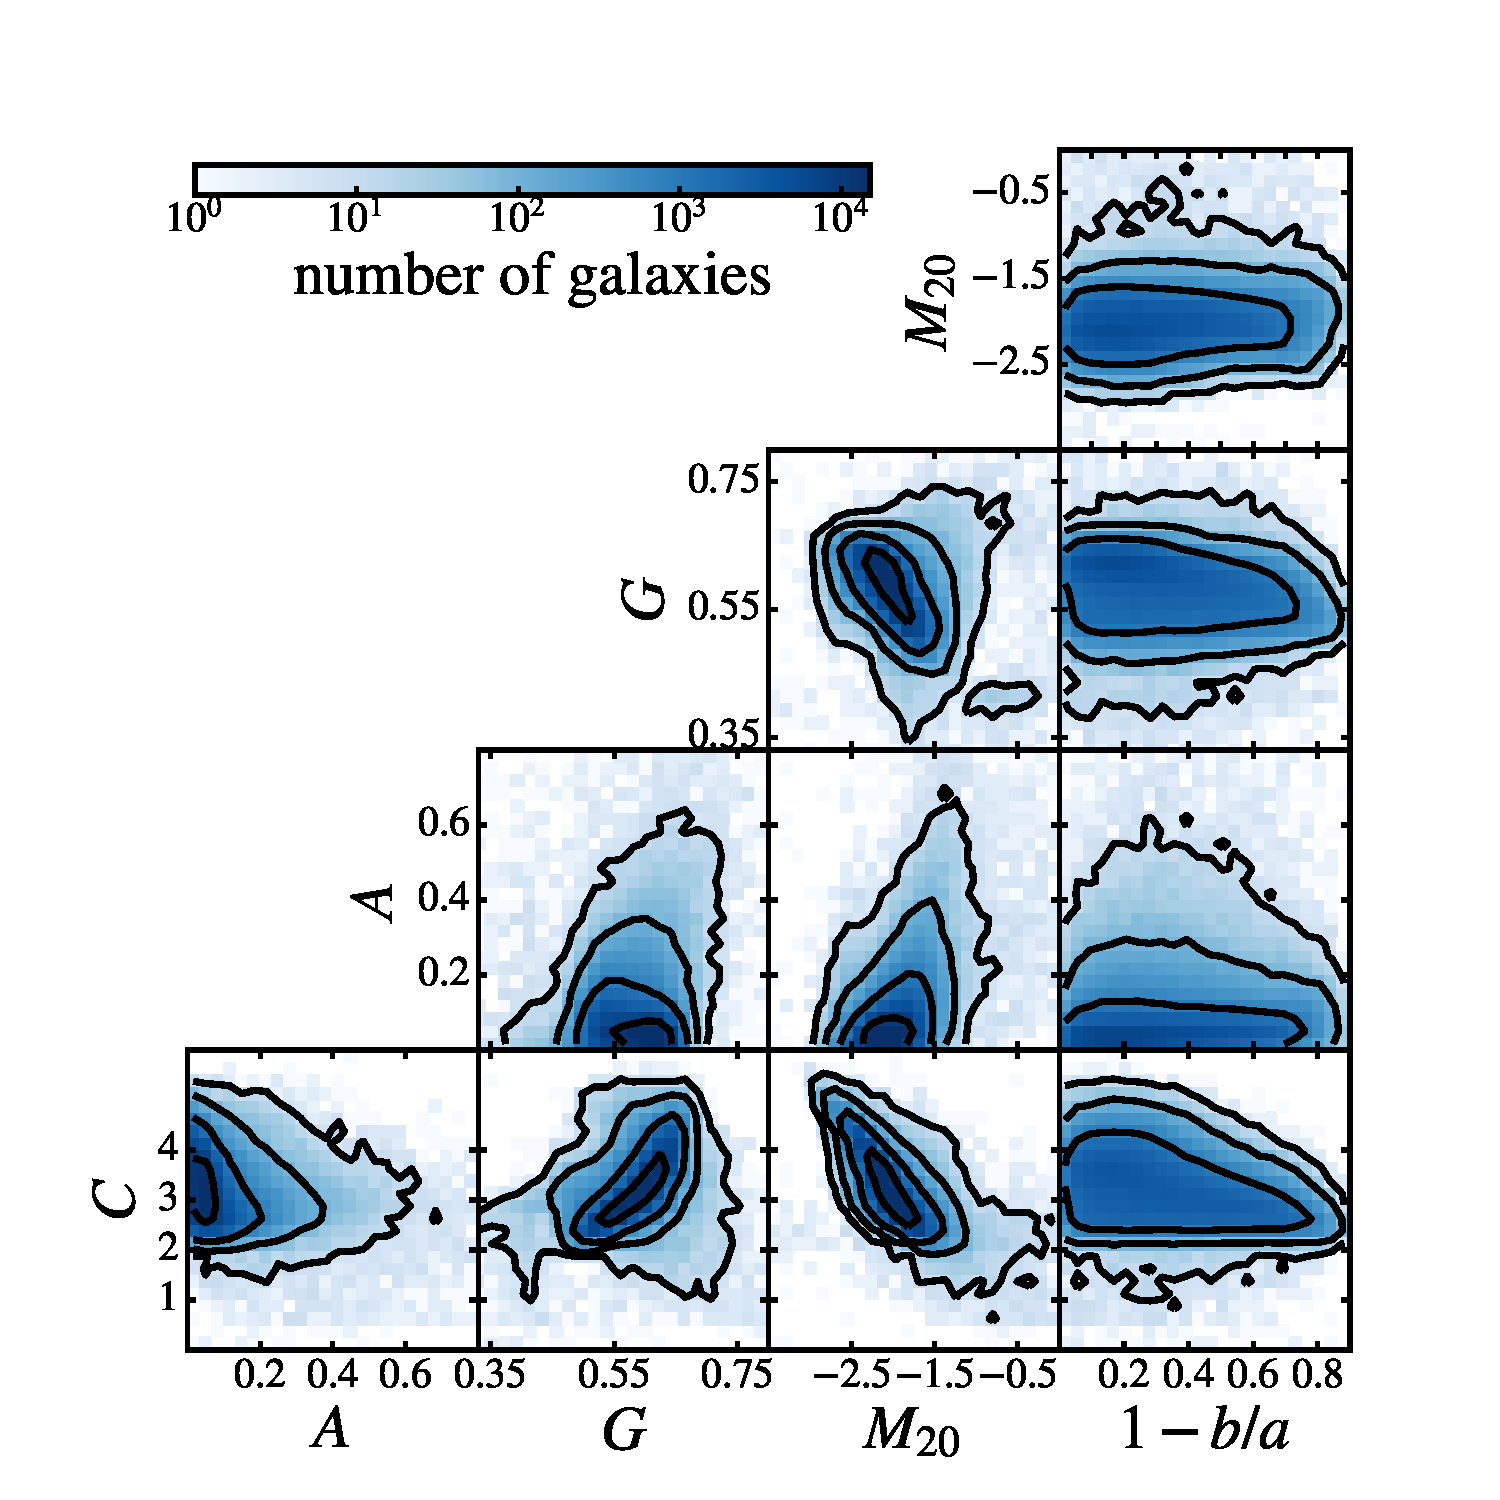
\includegraphics[width=3.7in]{Figures/human_machine/A2b.pdf}
\caption{\textit{Left.} Identifying~\feat~subjects is independent of identifying~\notfeat~subjects.  Both ROC curves use all subjects processed by SWAP where the score used to create the ROC curve is simply each subject's achieved posterior probability. The Featured curve demonstrates how well we identify~\feat~subjects with a threshold of 0.99, while the Not Featured curve demonstrates how well we identify~\notfeat~subjects with a threshold of 0.004. Typically, best performance is achieved by the score associated with the upper-left-most part of the curve. Our~\feat~threshold is nearly optimal, while our~\notfeat~threshold could be improved since the blue square is not as close to the upper left hand corner as other possible values of the subject posterior. \textit{Right.} Relation between measured morphology diagnostics for more than 280K SDSS galaxies. Most of these galaxies are processed through SWAP, receiving a posterior probability that estimates how likely each is to be~\feat~or~\notfeat.}
\label{fig: morph thresh}
\end{figure*}